%\PassOptionsToPackage{table}{xcolor}
\documentclass{beamer}
\usepackage{times,helvet,epsfig,color}
\usepackage{graphicx}
\usepackage{comment}
\usepackage{xspace}
\usepackage{hyperref}
%\PassOptionsToPackage{usenames}{xcolor}
\usepackage{overpic}
\graphicspath{{../img/}}
\mode<presentation>
{
	\usetheme{default} % I sometimes also use Warsaw
	\setbeamertemplate{itemize items}[circle]
	\setbeamertemplate{navigation symbols}{}
}
\setbeamertemplate{footline}
{
  \leavevmode%
  \hbox{%
  \begin{beamercolorbox}[wd=.3\paperwidth,ht=2.25ex,dp=1ex,left]{?}%
\hspace{1mm}
% \includegraphics[width=0.15\paperwidth]
%    {../../../current-docs/CarletonWide_K_186.png}
  \end{beamercolorbox}%
  \begin{beamercolorbox}[wd=.4\paperwidth,ht=2.25ex,dp=1ex,center]{title in head/foot}%
{\em 3D GREIT}, Grychtol, M\"uller, Adler, 2015/06/03
  \end{beamercolorbox}%
  \begin{beamercolorbox}[wd=.3\paperwidth,ht=2.25ex,dp=1ex,right]{title in head/foot}%
    \insertframenumber{}~/~\inserttotalframenumber\hspace*{1ex}
  \end{beamercolorbox}}%
  \vskip0pt%
}


\usepackage{tikz}
\pgfdeclarelayer{foreground}
 \pgfdeclarelayer{background}
 \pgfsetlayers{background,main,foreground}

\begin{document}


\title[3D GREIT]{
\vspace{10mm}
~\\
\Huge
{\em 3D Image Reconstruction with GREIT}
\\
\vspace{10mm}
}
\author{Bart\l{}omiej Grychtol$^1$,
Beat M\"uller$^2$, and
Andy Adler$^3$}
\institute[]{$^1$Fraunhofer Project Group for Automation in Medicine and 
Biotechnology, Mannheim, Germany 
\\
$^2$Swisstom AG, Landquart, Switzerland 
\\
$^3$Systems and Computer Engineering, Carleton University, Ottawa, Canada}
\date{}

\frame{\titlepage} 

\frame{\frametitle{%
GREIT \ldots
}

}

\frame{\frametitle{%
Reconstructions
}
\centering
\includegraphics[width=.4\columnwidth]{sigmoid_01a.png}
\hfill
\includegraphics[width=.4\columnwidth]{sigmoid_01b.png}
\\
Plots of the function $f(x) = 1 / (1 + e^{s(|x|-R)})$ for different values 
of $s$ with the default value indicated in bold.
}


\frame{\frametitle{%
Electronics -- Block Diagram
}
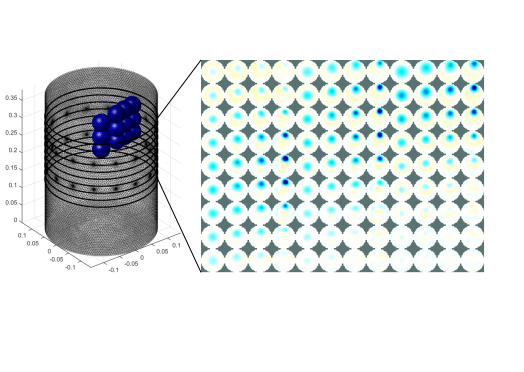
\includegraphics[width=\columnwidth]{tank_recon.pdf}
\\
\emph{Left:} FE model of a water tank showing 
cut planes between voxel layers and positions of a non-conductive spherical 
target. \emph{Right:} images reconstructed using the proposed algorithm. Each 
row corresponds to one voxel layer, and each column to a different target 
position.
}



\end{document}

